\chapter{Introduction \& Background}
Alright, so the thing that is on everybody's mind is probably: what is an atomic 
swap? An atomic swap is where two parties exchange assets atomically, which means
that either the transaction takes place fully, or the state is reset to the pre-
exchange state. 

*Read from oracle defenition*

This is made possible by clever use of cryptography and 
programmable contracts on the bitcoin network and blockchain. So before we can 
go into more detail on this I should first cover the basics of Bitcoin.

So, most people, especially in computer science, have heard of Bitcoin, but I could 
almost count on one hand the number of people I have met that have more than 
a basic understanding of how it works. I could talk for hours about this 
subject, but sadly there is no time for that. So I will try to give you the 
shortest possible version where you can at least understand the rest of my
thesis.

The simplest description of Bitcoin is a shared public ledger, that relies 
on proof-of-work to build network-wide consensus. First of proof-of-work
is a way to prove mathematically that work was put into doing something. 
The most common way of doing this is via hashing of some datatype.
The hash has to meet certain criteria to be accepted. There is no known 
way of producing a wanted hash, so the only way is to try different combinations
until a good result is found. So if you have data that produces a certain hash
that hash serves as proof that you put work into creating it.

Another thing you have probably heard about before is the blockchain, but
just as with Bitcoin overall, people know little about what it actually is. 
A blockchain is basically a shared datatype. It is very reminiscent of a
linked list, but allows for branching, meaning that two elements can link 
to the same parent. We will come back to this in a moment, but first, let's 
take a closer look at the blocks.

A block is a data structure that has a header and data. The header contains 
metadata about the block itself as well as a reference to the previous block
in the chain. In Bitcoins case, the data in the block is just a list of transactions,
but you could put anything you want into this field. The reference to the previous
block is what forms the chain. You can from any block follow the references 
all the way back to the original block. Anyone can add a block to the chain. But 
it has to meet the proof-of-work criteria. The Bitcoin network independently calculates 
something called mining-difficulty. This is represented by a large 256-bit number. 
For your new block to be accepted the header of the block has to produce a hash that
is strictly smaller than the difficulty number. You produce unique hashes by changing 
a field in the header called nonce, this process is what is referred to as mining. 

The mining-difficulty is set so that the sum of all participant's hash-calculating power,
or hashrate, will produce  new block on average every 10 minutes. The difficulty is adjusted 
every 2016th block. 

So how does proof-of-work ensure that the shared ledger stays consistent? This is
where concepts like longest chain comes in. The Bitcoin network only accepts the longest
chain as truth, in other words the chain with most accumulated proof-of-work. 
This works as long as the majority of participants is honest. However due to the
probabilistic manner of how new valid blocks are found there is still a chance for 
contention even if all participants are honest. For example what will the network do
in the case where two different blocks are found at almost the same time, in 
different parts of the network? Now 
there are two chains of equal length. So how does the network decide which one
is correct?

*Explain pictures*

%https://en.bitcoin.it/wiki/Transaction
%mastering bitcoin
\Section{Transactions}\label{transactions}
Transactions in Bitcoin are not as straight forward as you might expect a transaction to be. A transaction contains a list of inputs and a list of outputs as well as some metadata like version number and lock-time.\cite{bitcoin_core_tx}\cite{antonopoulos_2017}

\begin{figure}[H]
	\centering
	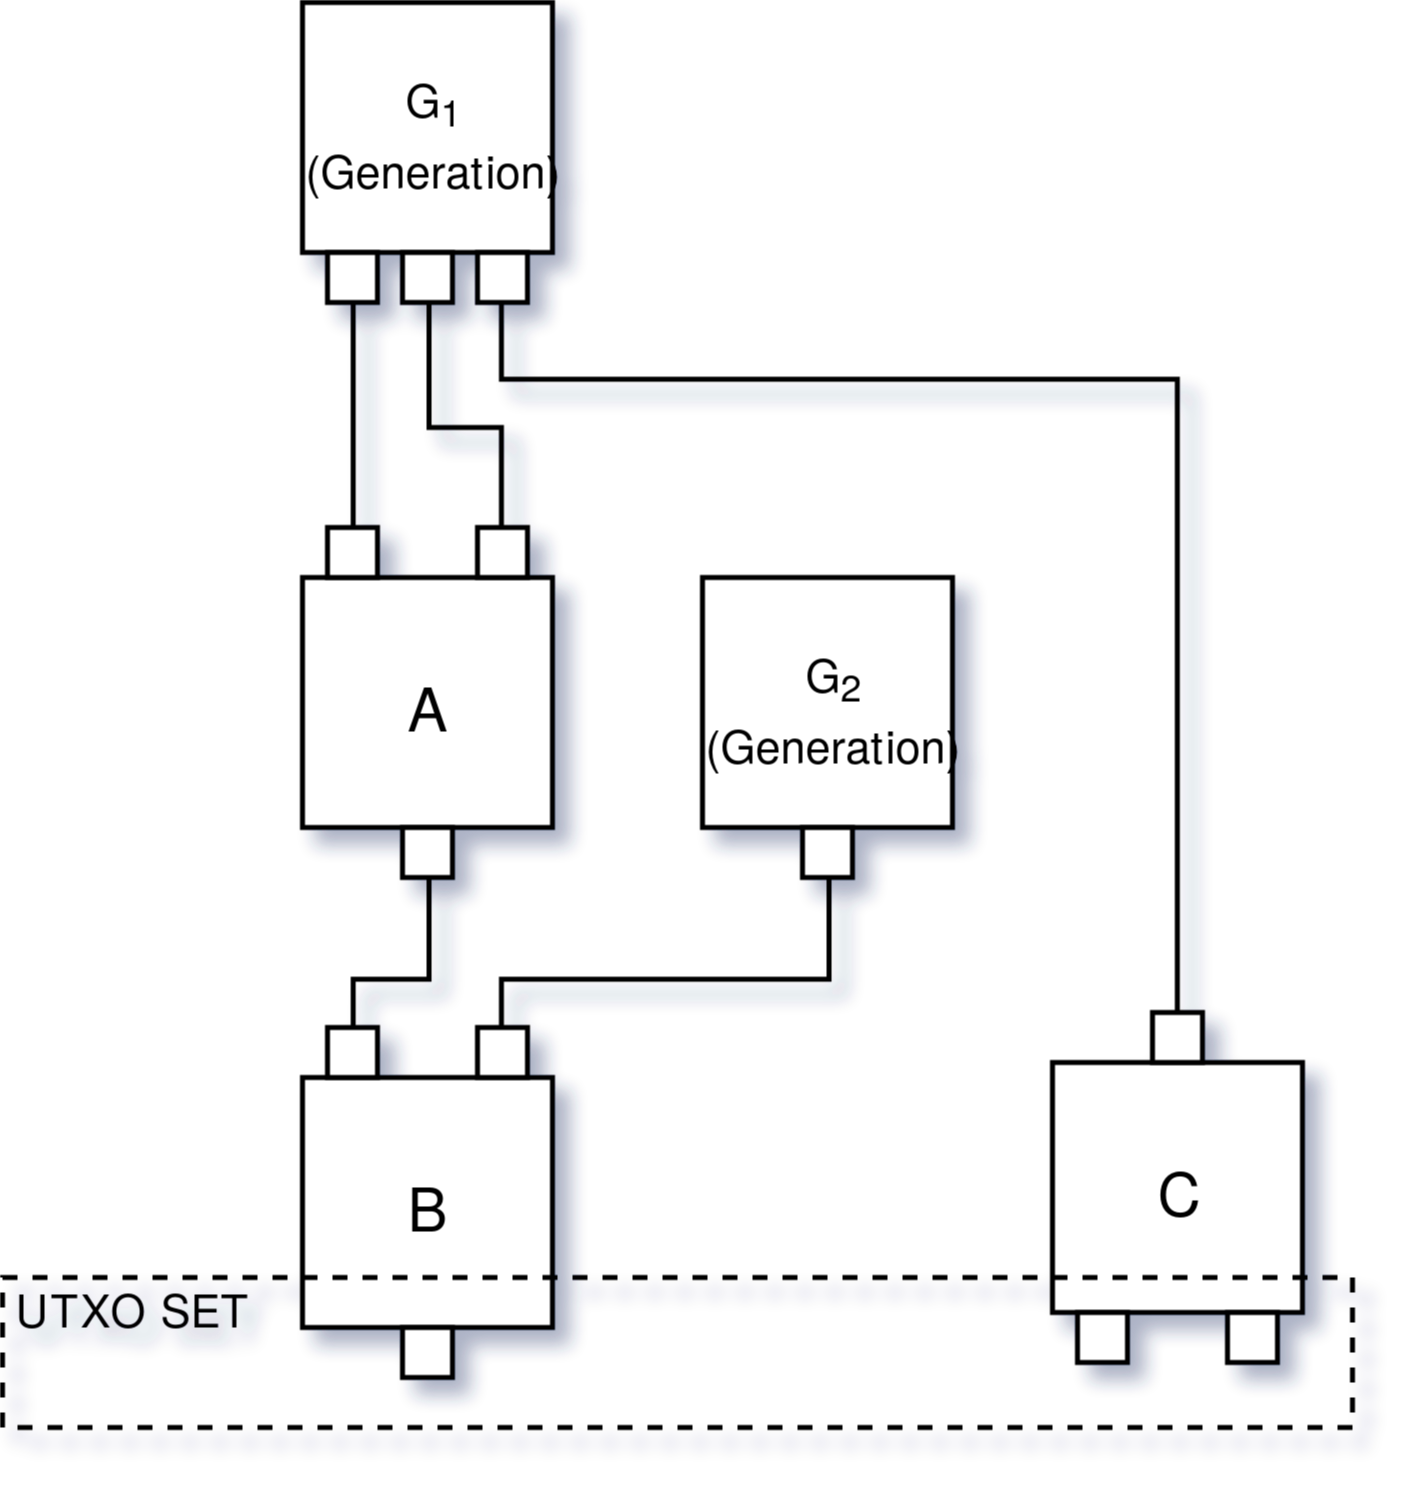
\includegraphics[width=0.75\textwidth]{background/images/transaction_diagram.png}
	\caption{4 example transactions and how inputs are connected to outputs}
	\label{fig:transaction_input_output}
\end{figure}

In simplified terms an output could be seen as the destination of a transaction, in other words it says how much and to whom the transaction is sent to. An input is a reference to a previous output. The inputs take the money from the outputs they reference and that money is used to fund the new outputs.\cite{antonopoulos_2017}\cite{bitcoin_core_tx}

The inputs and outputs is where Script comes into the picture. Both outputs and inputs contains an incomplete script, together however they complete the script. The script in an output could be seen as a challenge, and the script in the input is the response. When a transaction is tested for validity the input script is appended to the script in the output and is executed. If the script comes out as valid the transaction is also valid.\cite{antonopoulos_2017}\cite{bitcoin_core_tx} Here is a basic example: Let's say Alice wants to send a transaction to whoever can answer the equation $4+3$. Her transaction output would contain the script:

\texttt{4 3 OP\_ADD OP\_EQUALS}

If this is executed as is it is invalid. But let's say Bob knows the answer to the equation he can then create a new transaction where the input contains the script: 

\texttt{7} 

Just as before this script is not valid by itself. But then the transaction is checked for validity the input will be appended to the start of the output script forming the following: 

\texttt{7 4 3 OP\_ADD OP\_EQUALS}

Which is a valid script, thus Bobs new transaction is also valid and he may spend the money as he see fits. 

Obviously most transactions on the Bitcoin blockchain are not this simple. The most common form of transaction contains a script called P2PKH which stands for Pay to public key hash. Before we can go into details on this one however we first need to know about how signatures and sighash work in script and transactions.

\Subsection{Signatures and sighash}
Section \ref{ecdsa} covers public keys and signatures in depth.

Perhaps the most important operation in script is the \texttt{OP\_CHECKSIG} operation and its cousins. \texttt{OP\_CHECKSIG} pops two values from the stack, if the script is correctly implemented these two values should be the public key and a signature created with the private key that correlates with mentioned public key

The question is: what is signed when the signature is created? Broadly speaking it is the hash of the transaction that is trying to spend the output, this is not entirely accurate however.\cite{antonopoulos_2017} Appended to the signature that is a flag called \textbf{sighash} (Signature hash). The value of sighash tells the script interpreter what hash was signed during the creation of the signature.\cite{bitcoin_core_sighash} There are 4 types of sighash implemented:

\Subsubsection{SIGHASH\_ALL}
This can be considered the default sighash, if it is not stated otherwise it can safely be assumed that this type was used. This simply means that the entire transaction is signed with all outputs and all other inputs.

\Subsubsection{SIGHASH\_NONE}
This one signs the transaction but without the outputs, it could be thought of as ''I don't care where the money goes''.

\Subsubsection{SIGHASH\_SINGLE}
All outputs are removed except the output with the same index as the input that is being signed, then that transaction is signed.
This could be thought of as ''I dont care about any other outputs to this transaction as long as this one remains as is''.

\Subsubsection{SIGHASH\_ANYONECANPAY}
Signs the transaction with all the outputs but none of the other inputs. This basically means ''The money has to go here, but I don't care if someone else want to fund this transaction also''

%\Subsubsection{More detailed process}
%On the next page the entire signing process for SIGHASH\_ALL is detailed. This is how it is performed in the actual implementation:
%\newpage
%\centerline{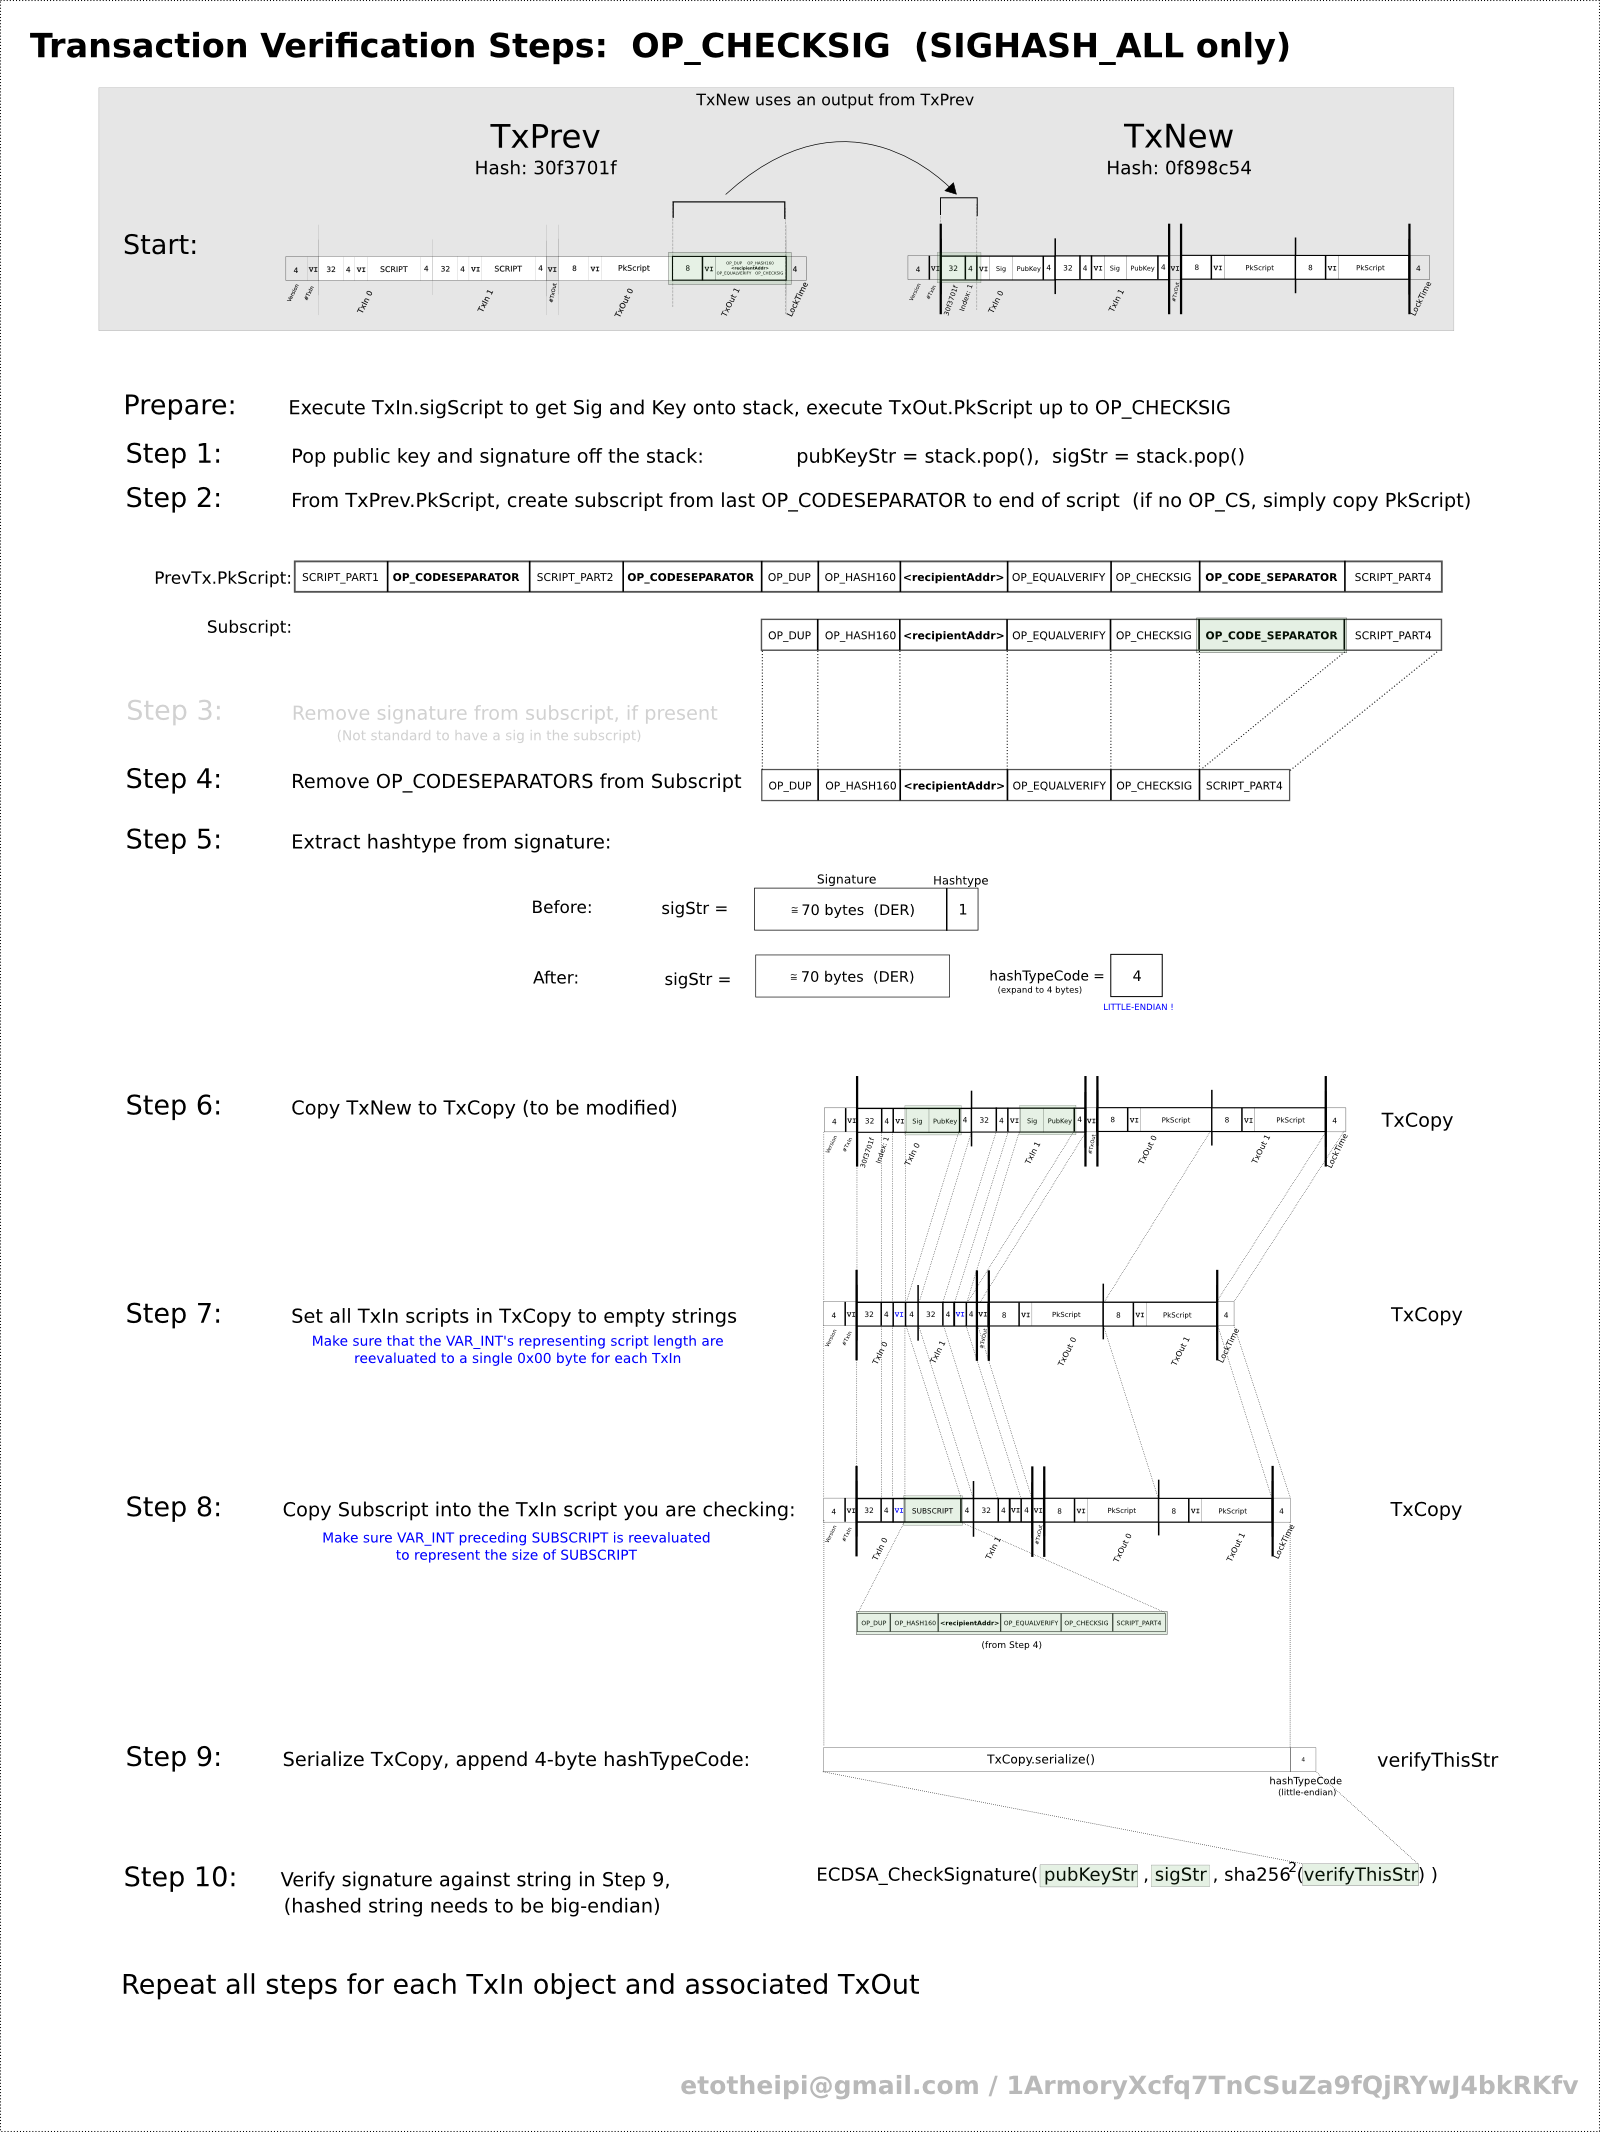
\includegraphics[width=1.35\textwidth]{background/images/checksig_in_detail.png}}
%\newpage

\Subsection{Pay to public key hash (P2PKH)}\label{p2pkh}
P2PKH is as mentioned the most common form of transaction.\cite{antonopoulos_2017} This transaction can be thought of as paying to somebodies address. In other words the output of this transaction contains a script where the one who wants to redeem it must prove that they own the private key which created the public key the address is referring too. This is what the script looks like in the output:

\texttt{OP\_DUP OP\_HASH160 <public key hash> OP\_EQUALVERIFY OP\_CHECKSIG}

As mentioned already executing the script in the output by it self doesn't make any sense, especially now when the very first operation \texttt{OP\_DUP} tries to duplicate the top element in the stack. But at execution the stack will be empty. Anyone wanting to spend this output would construct a transaction with the input script on the following form:

\texttt{<signature> <public key>}

When the input and output is executed together the process goes like this: 
\begin{enumerate}
	\item First the signature and unhashed public key is pushed to the stack.
	\item The public key is duplicated (there are now one signature and two public keys on the stack).
	\item The top public key goes through the HASH160 process making it a hashed public key.
	\item The hashed public key from the output is pushed on the stack, at this point the stack has the following elements (\texttt{<signature>}, \texttt{<public key>}, \texttt{<hashed public key>}, \texttt{<hashed public key>}).
	\item \texttt{OP\_EQUALVERIFY} checks if the top two elements is equal and verifies the result, What basically has been done is is that the script checks if the public key provided in the input script is equal to the hashed public key given in the output script.
	\item At this point the stack has the following elements: (\texttt{<signature>}, \texttt{<public key>}). \texttt{OP\_CHECKSIG} pops these from the stack and checks if the signature is valid.
\end{enumerate}

In the early days of bitcoin you payed directly to public keys instead of hashed public key. The reason the hash part was added at all has to do with extra security. If an exploit is found in elliptic curve cryptography that makes it so someone could calculate the private key from a public key then all unspent outputs would be at risk of being stolen. With the hashed public key the actual public key is not revealed until the output is spent, and then it is too late for it to be stolen. This of course requires that everyone uses a different public key for every transaction, which is the standard today.\cite{bitcoin_core_tx}

\Subsection{Pay to script hash (P2SH)}
Pay to script hash is slightly newer and a bit more complex to understand. Instead of paying to someones address, you pay to a script, this was initially proposed by Gavin Andreasen in 2012.\cite{scripthash} Let's say Alice has partial script S, that can be solved with the partial script K. She can then hash S and get $H_S$. She then creates transaction with an output containing the following script:

\texttt{OP\_HASH160 <$H_S$> OP\_EQUAL}

If Bob wants to redeem this transaction he first has to know the script and how to solve it. This is how the transaction input would look like: 

\texttt{K <S>}

The execution of the combined input output script is not straight forward as most scripts are. This is the process:
\begin{enumerate}
	\item The K part of the script is executed as usual. This pushes or does whatever it needs to do to make K + S a valid script.
	\item The partial script S is pushed to the stack in the form of bytes.
	\item This is where the execution takes a strange and not so intuitive path, as you will see. First the script is hashed with the \texttt{OP\_HASH160} operation.
	\item The script hash from the output is pushed on the stack.
	\item OP\_EQUAL checks if the top two items on the stack are equal. If they are it means that the script S provided in the input is the correct script.
	\item Unique to P2SH, the execution goes back to the original script S that was pushed to the stack in stage 2. And executes it together with whatever K pushed to the stack. This script also has to be valid.\cite{scripthash} 
\end{enumerate}

If all stages are executed without error the redeeming transaction is valid. 

P2SH was developed to resolve the difficulties in making complex transaction scripts and make them as simple as paying to an address. What P2SH basically means is ''pay to a script matching this hash, a script that will be presented later when this output is spent''\cite{antonopoulos_2017}\cite{scripthash}

\Subsection{Timelock and sequence}
Since the start of bitcoin; transactions has had two fields in them called \textbf{nTimelock} and \textbf{nSequence}. The timelock variable stopped a transaction from being  included in a block until a certain unix-timestamp or a certain blockheight\footnote{Blockheight is the number of blocks on the current chain} had passed. The sequence field is part of each input into a transaction, it's original purpose was to give users a mechanism for updating a transaction that were still in the transaction-pool. Miners were supposed to include the transaction version with highest sequence number, this however was unenforceable, as there is no way of knowing which transactions were in the transaction-pool of the miner at the time of block creation. So nSequence became mostly defunct and saw little use.

To make timelocks more versatile and more easily enforceable Peter Todd proposed an addition to Script, a new op-code that verifies that the correct timestamp is set, \\\texttt{OP\_CHECKTIMELOCKVERIFY}.

As timelocks only allows for absolute wait time, like for example: ''this transaction can only be spent after \texttt{10th June 2019}''. Mark Friedenbach et al. proposed in 2015 to add an additonal op code to Script that can check for relative time passage as well, \texttt{OP\_CHECKSEQUENCEVERIFY}.

\Subsubsection{OP\_CHECKTIMELOCKVERIFY}
There is an operation in Script called \texttt{OP\_CHECKTIMELOCKVERIFY}, what it does is that it compares the timestamp or blockheight that is on the stack and compares it to the timestamp that is in the transaction trying to spend the output that this op code is part of.\cite{antonopoulos_2017}\cite{checklocktime}\cite{script_wiki}\cite{bitcoin_core_tx}

\Subsubsection{OP\_CHECKSEQUENCEVERIFY}
\texttt{OP\_CHECKSEQUENCEVERIFY} is a lot like the previous one except it it deals with relative time. 

Let's say you have two transactions transaction $T_A$ and transaction $T_B$, $T_A$ is included in a block on the blockchain. If $T_B$ tries to spend one of $T_A$ outputs and has that specific input marked with a  sequence of 10. It means that $T_B$ can't be included in the block chain until $T_A$ is at least 10 blocks deep in the blockchain.\cite{antonopoulos_2017}\cite{checksequence}\cite{script_wiki}\cite{bitcoin_core_tx}

\texttt{OP\_CHECKSEQUENCEVERIFY} enforces this in the output. If $T_A$ has \texttt{10 OP\_CHECKSEQUENCEVERIFY}, then if $T_B$ tries to spend that output it has to be at least 10 blocks deep.

